\section{Versuchsaufbau}
Die gesamte Messschaltung ist in Abbildung \ref{fig:Mess} abgebildet.
Der Kern des Versuchsaufbaus ist aber die Franck-Hertz-Röhre wie Sie in Abbildung \ref{fig:FH} abgebildet ist. Sie ist ein
mit Hg-Dampf gefülltes Glasrohr. In ihr befindet sich ein Heizfaden, der an eine Gleichspannungsquelle
angeschlossen wird. In der Mitte der Röhre ist eine netzförmige Beschleunigungselektrode angeschlossen.
Zwischen Heizfaden und Beschleunigungselektrode können Gleichspannungen bis zu 60V angeschlossen werden.
Auf der gegenüberliegenden Seite zum Heizfaden ist die Auffangelektrode installiert.
Zwischen Beschleunigungselektrode und Auffangelektrode können Spannungen bis zu 11V angeschlossen werden.
Beide Spannungen sind an einem Gerät angeschlossen, dass die Spannung automatisch zeitproportional 
steigen und fallen lassen kann. Zur Einstellung des Innendrucks ist ein Temperaturregler
an das heizbare Blechgehäuse der Franck-Hertz-Röhre angeschlossen. Über ein Thermometer 
kann die Innentemperatur des Gehäuses überprüft werden. Der Strom, der 
an der Auffangelektrode ankommt, wird mit einem Picoamperemeter gemessen. Um nun den 
Auffangstrom für verschiedene Beschleunigungsspannungen oder Bremsspannungen aufzuzeichnen,
kann ein X-Y-Schreiber angeschlossen werden. Dafür wird die entsprechende zu variierende Spannung auf den X-Eingang
des Geräts gelegt und der Strom auf den Y-Eingang.
\begin{figure}[H]
    \centering
    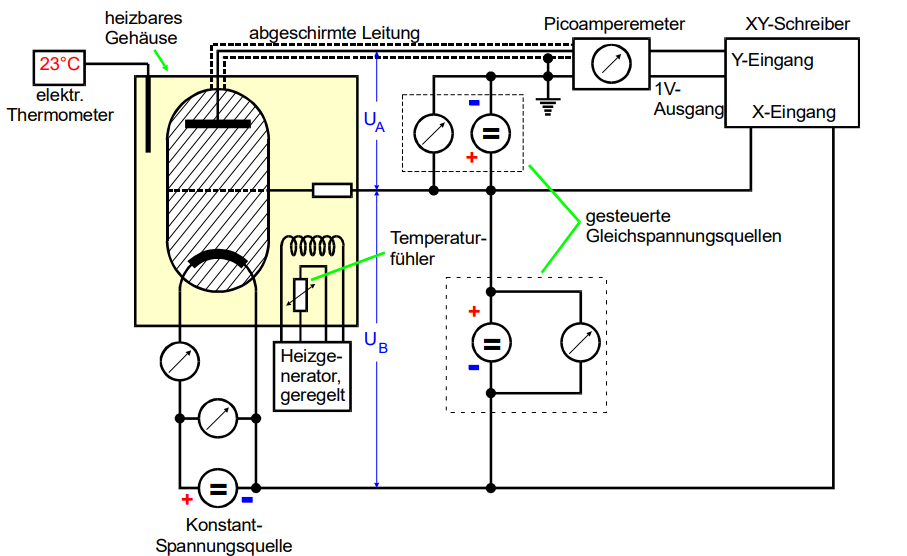
\includegraphics[scale=0.8]{content/Messschaltung.png}
    \caption{Schaltung zur Aufnahme einer Franck-Hertz-Kurve \cite{sample}.}
    \label{fig:Mess}
\end{figure}
\subsection{Kalibrierung des X-Y-Schreibers}
Integraler Bestandteil aller korrekten Messungen mit der Apparatur, ist die richtige Kalibrierung 
des X-Y-Schreibers. Der erste Schritt nach Einlegen eines Blattes und der elektrostatischen Fixierung ist 
die Kalibrierung der Y-Achse. Zunächst wird kein Strom auf den Schreiber gelegt und der Nullpunkt soweit
verschoben bis der Stift am unteren Rand des Millimeterpapiers ansetzt. Nun wird die gesamte Messschaltung so eingestellt,
dass der größtmögliche Strom, der während der gewünschten Messung bei gleichen Rahmenbedingungen erzeugt werden kann, am 
Schreiber ankommt. Damit soll das Maximum kalibriert werden. Die Skalierung wird dabei so verändert, dass der Ausschlag am oberen Ende 
der Apparatur liegt. Nun kann der Anschluss des Picoamperemeters zunächst vom Schreiber getrennt werden und die X-Achse wird kalibriert.
Dafür wird zunächst wieder der Nullpunkt ohne angeschlossene Spannung festgelegt. Dann wird bei größtmöglicher angeschlossener Spannung 
die Skalierung so eingestellt, dass der Vollausschlag am rechten Rand endet. Nun muss noch eine Skalierung zur 
Messung hinzugefügt werden, um signifikante Punkte einem Spannungswert zuordnen zu können. Dafür wird die Spannung 
stückweise reduziert und in regelmäßigen Abständen z.B. in 1V Abständen eine Markierung mit dem Stift des Schreibers gesetzt.
Ist die Spannung wieder im ursprünglichen Zustand, kann die eigentliche Messung beginnen. Beide 
Kanäle werden auf X und Y angeschlossen. Der Stift wird aufgesetzt und die Spannung kann zeitlich konstant erhöht werden.
\section{Versuchsdurchführung}
Als erstes soll die Energieverteilung der Elektronen, die sich aus dem Glühdraht lösen, bei Raumtemperatur 
und bei 140-160°C gemessen werden. Dafür wird eine konstante Beschleunigungsspannung eingestellt. Die Gegenspannung 
wird hingegen zeitproportional von 0 bis zum Maximalwert erhöht. Daher wird die Gegenspannung 
an den X-Kanal des X-Y-Schreibers angeschlossen. Nach der Kalibrierung des Schreibers kann 
der ankommende Auffangstromm in Abhängigkeit von der Gegenspannung aufgenommen werden. 
Nun soll die Messung bei 140°-160°C wiederholt werden. Dafür wird der Temperaturregler hochgedreht. 
Die Temperatur wird am Thermometer beobachtet und der Regler wird so verstellt, dass bei der gewünschten Temperatur ein Gleichgewicht vorliegt.
Nun kann die Messung wiederholt werden.\\
\\
\noindent Der zweite Teil der Messung beschäftigt sich nun mit der tatsächlichen Aufnahme von Frack-Hertz-Kurven.
Diese sollen im Temperaturbereich zwischen 160°C und 200°C aufgenommen werden. Es sollen je bei zwei verschiedenen Temperaturen Kurven 
mit zwei verschiedenen Gegenspannungen aufgenommen werden. Dabei sollen die Maxima möglichst gut ausgeprägt sein.
Nun muss zunächst die Temperatur mittels des Reglers erhöht werden. Bei den jeweiligen Temperaturen wird die Gegenspannung 
je einmal auf 1V und einmal auf 2V gestellt. Die Beschleunigungsspannung soll zwischen 0 und 60V erhöht werden.
Daher wird diese Spannung an den X-Y-Schreiber angeschlossen. Die Schaltung muss auch hier bei jeder Messung neu kalibriert werden. 
\label{sec:Durchführung}
